%
%!TEX root = ../../hp3D_user_guide.tex
%

\chapter{Model Problems}
\label{chap:examples}

%--------------------------------------------------------------------

%
%!TEX root = ../../../hp3D_user_guide.tex
%

%--------------------------------------------------------------------

\section{Poisson Problems}
\label{sec:poisson}

For the first model problem implementation, we consider the Poisson problem with inhomogeneous Dirichlet BC:
\begin{alignat*}{3}
	- \div \nabla u &= f && \quad \text{in } \Omega \, , \\
	u &= u_0 && \quad \text{on } \Gamma \, .
\end{alignat*}

Classical variational formulation:
\[
\left\{
\begin{array}{llll}
	u \in H^1(\Omega):  u = u_0 \text{ on } \Gamma \, , \\[5pt]
	(\nabla u, \nabla v) = (f,v) \, ,
	\quad v \in H^1(\Omega) \, : \, v = 0 \text{ on } \Gamma \, .
\end{array}
\right.
\]

\subsection{Galerkin implementation}
\label{subsec:poisson-galerkin}

The Galerkin FE implementation of the variational problem is located in the application directory \file{problems/POISSON/GALERKIN}. In the remainder of this section, file paths may be given as relative paths within the application directory.

Input files:
\begin{itemize}
	\item{\file{control/control}: sets global control variables, e.g.
	\begin{itemize}
		\item \var{NEXACT} $\in \{$ \code{0,1} $\}$: indicates whether the exact solution is known.
		\item \var{EXGEOM} $\in \{$ \code{0,1} $\}$: indicates whether isoparametric or exact-geometry elements are used.
	\end{itemize}
	}
	\item{\file{input/physics}: sets initially allocated nodes and physics variables.
\begin{lstlisting}[caption=\file{POISSON/GALERKIN/input/physics} input file.]
100000              MAXNODS, nodes anticipated
1                   NR_PHYSA, physics attributes
field   contin  1   H1 variable
\end{lstlisting}
	\begin{itemize}
		\item The value of \var{MAXNODS} does not have to be precise; if more nodes are needed, the code allocates them on-the-fly. However, it is recommended for efficiency that the code does not reallocate, as well as not selecting \var{MAXNODS} much larger than needed.
		\item \code{\var{NR\_PHYSA}=1} specifies that \emph{one} physics variable is declared.
		\item \code{`field   contin  1'} specifies ``nickname, approximation space, number of components'' of a variable. The approximation spaces are: $H^1$ -- \code{contin}, $H(\tcurl)$ -- \code{tangen}, $H(\tdiv)$ -- \code{normal}, $L^2$ -- \code{discon}.
		\item For this Galerkin FE formulation, one $H^1$ variable is needed.
	\end{itemize}
	}
	\item{\file{geometries/hexa\_orient0}: defines the initial geometry mesh (a cube).}
\end{itemize}

Next, we take a look at the required routines that must be provided by the user:
\begin{itemize}
	\itemsep 0pt
	\item
	{\routine{set\_initial\_mesh}:\\
	for \emph{each} initial mesh element, this routine sets
	\begin{itemize}
		\itemsep 0pt
		\item the supported physics variables;
		\item the initial polynomial order of approximation;
		\item the boundary condition flags for element faces on the boundary.
	\end{itemize}
\begin{lstlisting}[caption=\file{POISSON/GALERKIN/}\routine{set\_initial\_mesh} routine.]
!..loop over initial mesh elements
   do iel=1,NRELIS

!  ...1. set physics
      ELEMS(iel)%nrphysics = 1
      allocate(ELEMS(iel)%physics(1))
      ELEMS(iel)%physics(1) ='field'

!  ...2. set initial order of approximation
      select case(ELEMS(iel)%etype)
         case(TETR); Nelem_order(iel) = 1*IP
         case(PYRA); Nelem_order(iel) = 1*IP
         case(PRIS); Nelem_order(iel) = 11*IP
         case(BRIC); Nelem_order(iel) = 111*IP
      end select

!  ...3. set BC flags: 0 - no BC ; 1 - Dirichlet; 2-9 Custom BCs
      ibc(1:6,1) = 0
      do ifc=1,nface(ELEMS(iel)%etype) ! loop through element faces
         neig = ELEMS(iel)%neig(ifc)
         select case(neig)
            case(0); ibc(ifc,1) = 1
         end select
      enddo

!  ...allocate BC flags (one per component), 
!     and encode face BCs into a single BC flag
      allocate(ELEMS(iel)%bcond(1))
      call encodg(ibc(1:6,1),10,6, ELEMS(iel)%bcond(1))
   enddo
\end{lstlisting}
	}
	\item
	{\routine{dirichlet}:
	\begin{itemize}
	\item User-provided routine required by the system routine \routine{update\_Ddof} which computes the Dirichlet DOFs for element nodes (vertices, edges, faces) with a non-homogeneous Dirichlet BCs. 
	\item \routine{update\_Ddof} interpolates $H^1$, $H(\tcurl)$, $H(\tdiv)$ Dirichlet data using \emph{projection-based} interpolation.\footnote{\fullcite{demkowicz2008interp}}
	\item Required only if non-homogeneous Dirichlet BCs were set by the user in \routine{set\_initial\_mesh}.
\end{itemize}

\begin{lstlisting}[caption=\file{POISSON/GALERKIN/common/}\routine{dirichlet} routine.]
!  routine dirichlet: returns Dirichlet data at a point
!   in:   Mdle          - middle node number
!         X             - a point in physical space
!         Icase         - node case (specifies supported variables)
!   out:  ValH, DvalH   - value of the H1 solution, 1st derivatives
!         ValE, DvalE   - value of the H(curl) solution, 1st derivatives
!         ValV, DvalV   - value of the H(div) solution, 1st derivatives
subroutine dirichlet(Mdle,X,Icase, ValH,DvalH,ValE,DvalE,ValV,DvalV)
\end{lstlisting}
	}
	\item
	{\routine{elem}:
	\begin{itemize}
	\item User-provided routine that computes the element-local stiffness matrix and load vector.
	\item System module \module{assembly} provides global arrays for this purpose:
	\begin{itemize}
		\item \var{ALOC(:,:)\%array}: Element-local stiffness matrix.
		\item \var{BLOC(:)\%array}: Element-local load vector.
		\item These arrays are declared \omp{omp threadprivate} for shared-memory parallel assembly of different element matrices with OpenMP threading.
	\end{itemize}
\end{itemize}

\routine{elem} is called during assembly for each middle node \var{Mdle} in the \emph{active mesh}.

\begin{remark}
Constrained approximation, modification for Dirichlet nodes, and static condensation of element-interior (bubble) DOFs are automatically done afterwards by the system routine \routine{celem\_system} which provides the \emph{modified element} matrices to the assembly procedure.
\end{remark}

\begin{lstlisting}[mathescape,caption=\file{POISSON/GALERKIN/}\routine{elem} routine]
!..determine element type; number of vertices, edges, and faces
   etype = NODES(Mdle)%ntype
   nrv = nvert(etype); nre = nedge(etype); nrf = nface(etype)
   
!..determine order of approximation
   call find_order(Mdle, norder)
   
!..determine edge and face orientations
   call find_orient(Mdle, norient_edge,norient_face)
   
!..determine nodes coordinates
   call nodcor(Mdle, xnod)
   
!..set quadrature points and weights
   call set_3D_int(etype,norder,norient_face, nrint,xiloc,waloc)

!  ....... element integrals:

!..loop over integration points
   do l=1,nrint

!  ...coordinates and weight of this integration point
      xi(1:3) = xiloc(1:3,l); wa = waloc(l)

!  ...H1 shape functions (for geometry)
      call shape3DH(etype,xi,norder,norient_edge,norient_face, nrdofH,shapH,gradH)

!  ...geometry map
      call geom3D(Mdle,xi,xnod,shapH,gradH,nrdofH, x,dxdxi,dxidx,rjac,iflag)

!  ...integration weight
      weight = rjac*wa

!  ...get the RHS
      call getf(Mdle,x, fval)

!  ...loop through H1 test functions
      do k1=1,nrdofH

!     ...Piola transformation: $q \rightarrow \hat q$ and $\nabla q \rightarrow J^{-T} \hat \nabla \hat q$
         q = shapH(k1)
         dq(1:3) = gradH(1,k1)*dxidx(1,1:3) + &
                    gradH(2,k1)*dxidx(2,1:3) + &
                    gradH(3,k1)*dxidx(3,1:3)

!     ...accumulate for the load vector: $(f,q)$
         b_loc(k1) = b_loc(k1) + q*fval*weight

!     ...loop through H1 trial functions
         do k2=1,nrdofH

!        ...Piola transformation: $p \rightarrow \hat p$ and $\nabla p \rightarrow J^{-T} \hat \nabla \hat p$
            p = shapH(k2)
            dp(1:3) = gradH(1,k2)*dxidx(1,1:3) + &
                       gradH(2,k2)*dxidx(2,1:3) + &
                       gradH(3,k2)*dxidx(3,1:3)

!        ...accumulate for the stiffness matrix: $(\nabla p, \nabla q)$
            a_loc(k1,k2) = a_loc(k1,k2) + weight*(dq(1)*dp(1)+dq(2)*dp(2)+dq(3)*dp(3))

   enddo; enddo; enddo
\end{lstlisting}
	}
\end{itemize}

This concludes the list of necessary input files and routines required for defining the application code from the library-perspective. However, the user is encouraged to take a look at the remaining files within the \file{POISSON/GALERKIN} directory which include the driver \routine{main} and a variety of auxiliary files. In a future version of the user manual, we may include a discussion of these auxiliary files as well.

\subsection{DPG primal implementation}
\label{sec:poisson-primal}

Broken primal DPG formulation:
\[
\left\{
\begin{array}{llll}
	(u, \hat \sigma_n) \in H^1(\Omega) \times H^{-1/2}(\Gamma_h): u = u_0 \text{ on } \Gamma \, , \\[5pt]
	(\nabla u, \nabla v) - \lb \hat \sigma_n , v \rb_{\Gamma_h} 
	= (f,v) \, ,\quad v \in H^1(\Omega_h) \, .
\end{array}
\right.
\]

Compared to the Galerkin FE implementation, the primal DPG implementation mostly differs in the \routine{elem} routine. In practice, the DPG method is implemented in its mixed form \cite{demkowicz2017dpg} but the extra unknown---the Riesz representation of the residual---is statically condensed on the element level (see Appendix~\ref{chap:dpg}).

The implementation is provided in \file{problems/POISSON/PRIMAL\_DPG}.

Compared to the input files for the Galerkin implementation, the only change is in the \file{physics} file:
\begin{lstlisting}[caption=\file{POISSON/PRIMAL\_DPG/input/physics} input file.]
100000              MAXNODS, nodes anticipated
2                   NR_PHYSA, physics attributes
field   contin  1   H1 variable
trace   normal  1   H(div) variable
\end{lstlisting}
We now have specified two physics unknowns---$u$ and $\hat \sigma_n$, i.e.~\code{\var{NR\_PHYSA}=2}. The additional trace unknown $\hat \sigma_n$ is declared as an $H(\tdiv)$ variable in the \file{physics} file; the normal trace $\hat \sigma_n$ must later be specified as such by setting \code{\var{PHYSAi(2)}=.true.} (e.g.~in the \routine{main} driver).

The \routine{elem} routine for DPG formulations can be structured into three distinct steps:
\vskip 5pt

\begin{minipage}{0.48\textwidth}
\begin{enumerate}
	\itemsep -10pt
	\item Element integration \vspace{-15pt}
	\begin{itemize}
		\itemsep -8pt
		\item Stiffness: $\mr B$
		\item Load: $\mr l$
		\item Gram matrix: $\mr G$
	\end{itemize}
	\item Boundary integration \vspace{-15pt}
	\begin{itemize}
		\itemsep -8pt
		\item Stiffness: $\mr{\hat B}$
	\end{itemize}
	\item Constructing DPG linear system \vspace{-15pt}
	\begin{itemize}
		\itemsep -8pt
		\item Dense linear algebra
		\item {Statically condensed system\\[-5pt] 
		stored in \var{ALOC}, \var{BLOC}}
	\end{itemize}
\end{enumerate}
\end{minipage}%
\begin{minipage}{0.48\textwidth}
\begin{figure}[H]
	\centering
	\begin{subfigure}[b]{0.6\textwidth}
		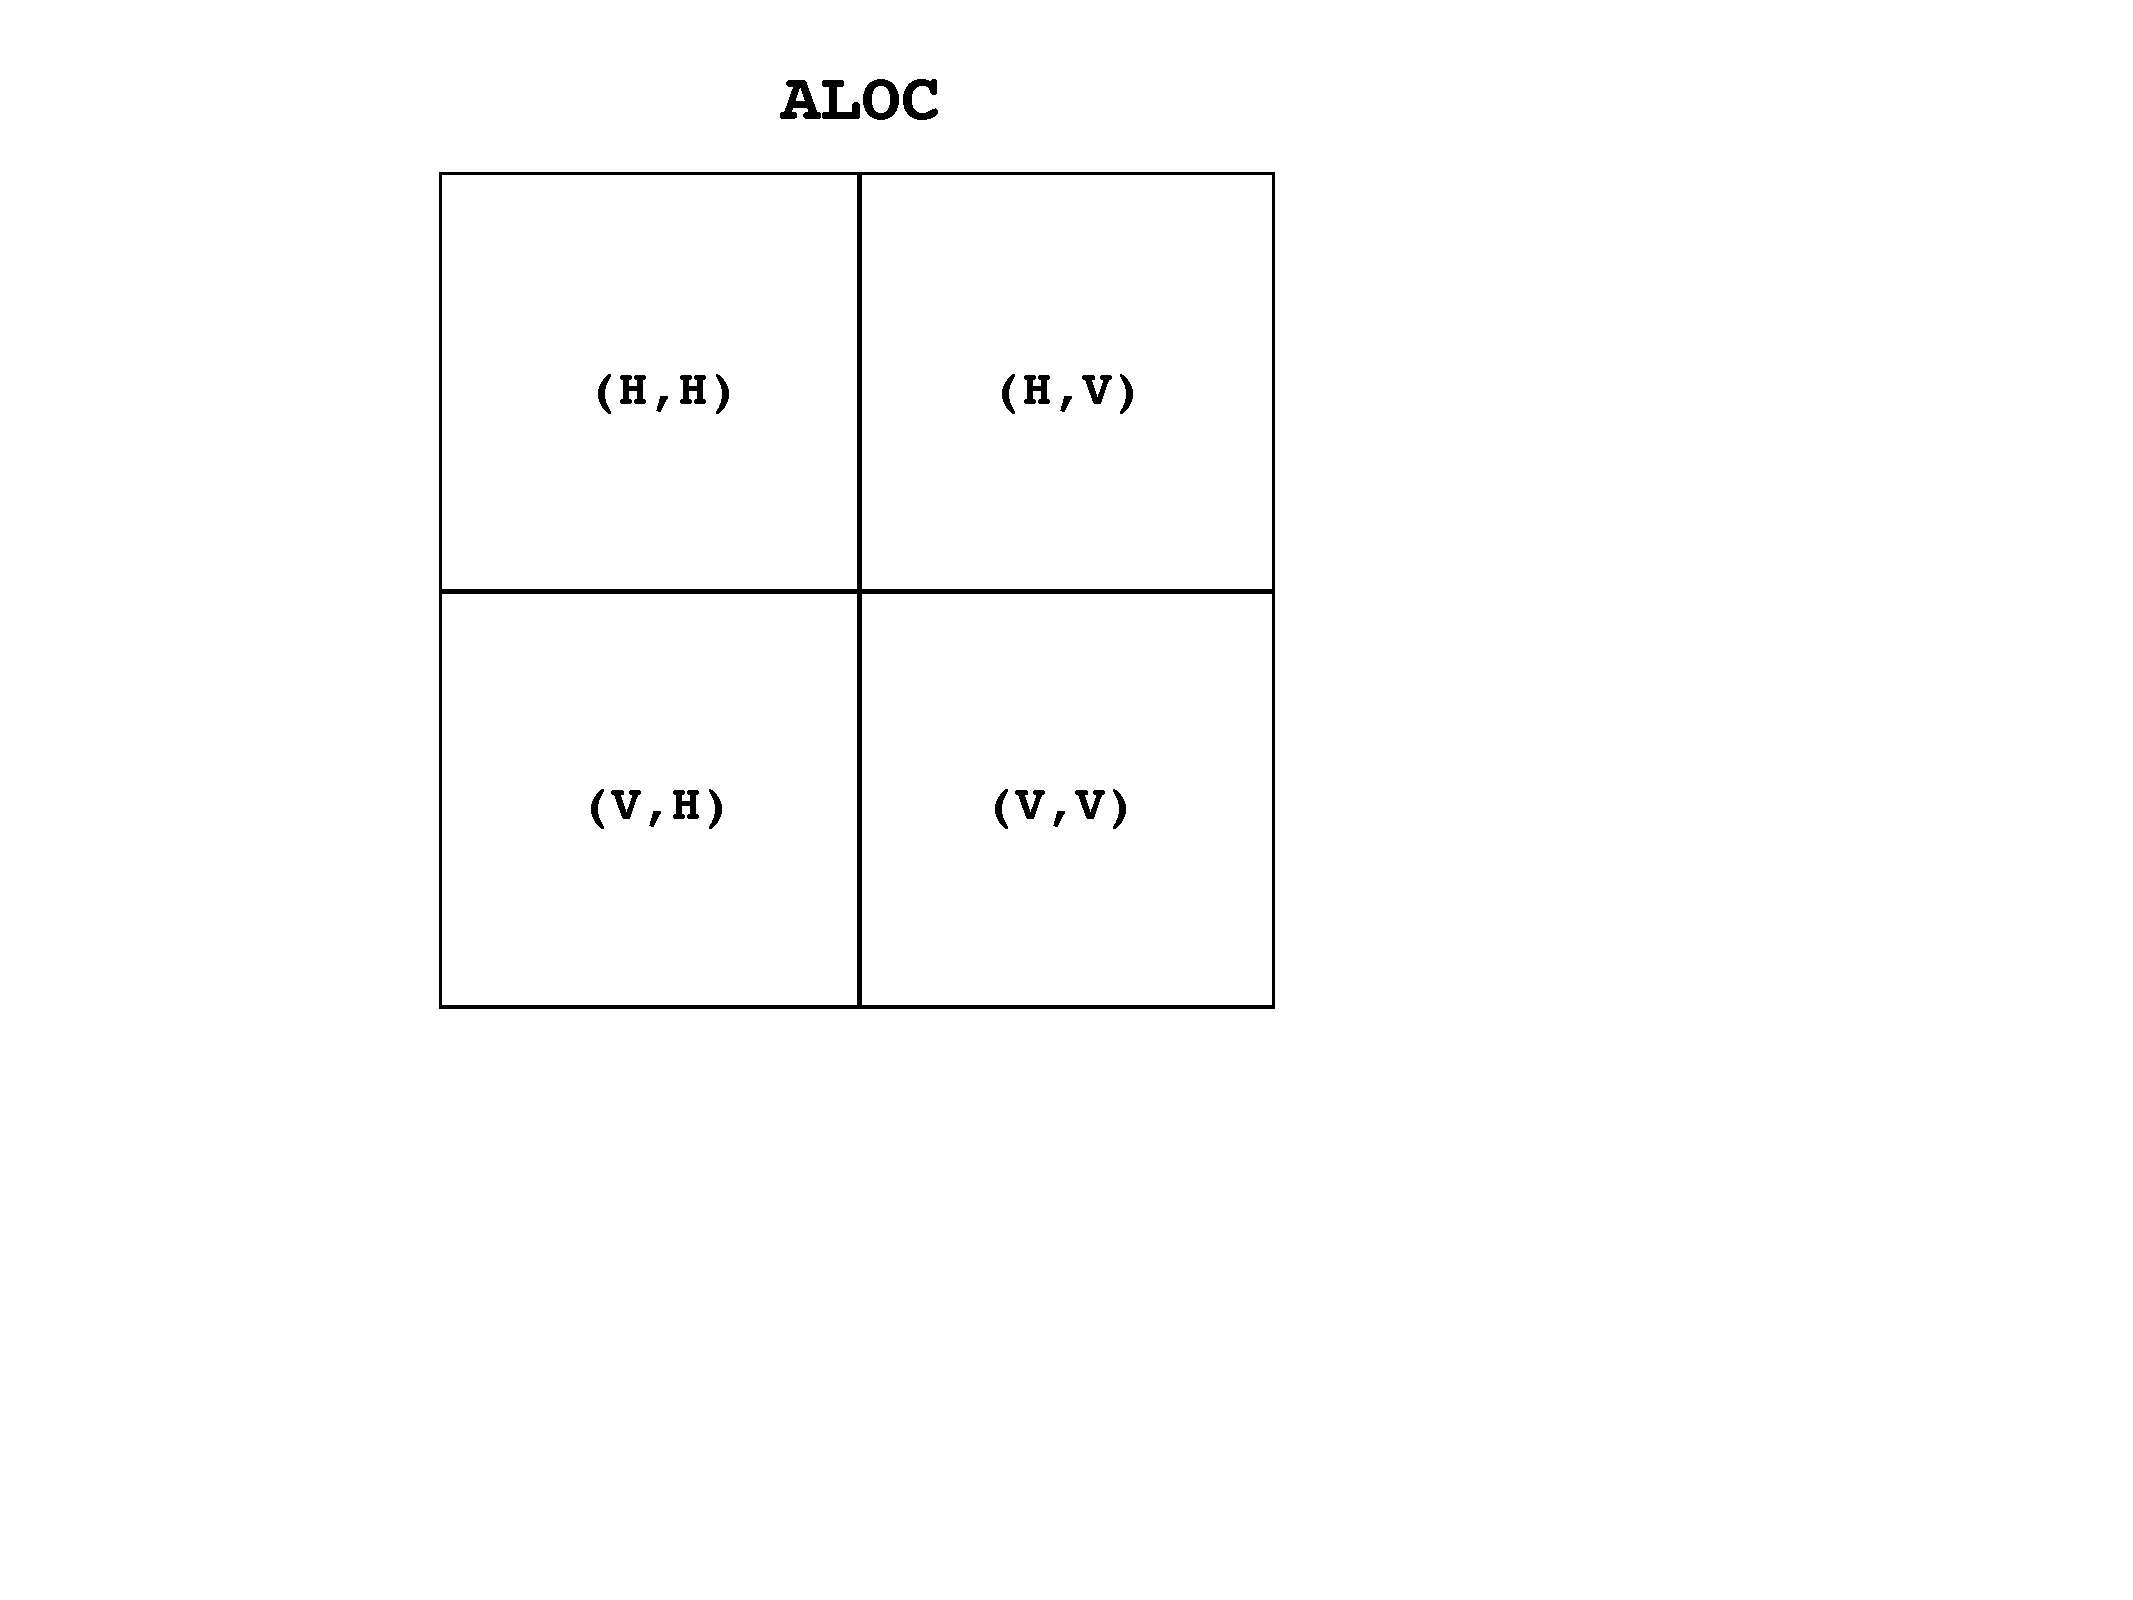
\includegraphics[height=1.8in]{ALOC.pdf}
	\end{subfigure}
	\begin{subfigure}[b]{0.3\textwidth}
		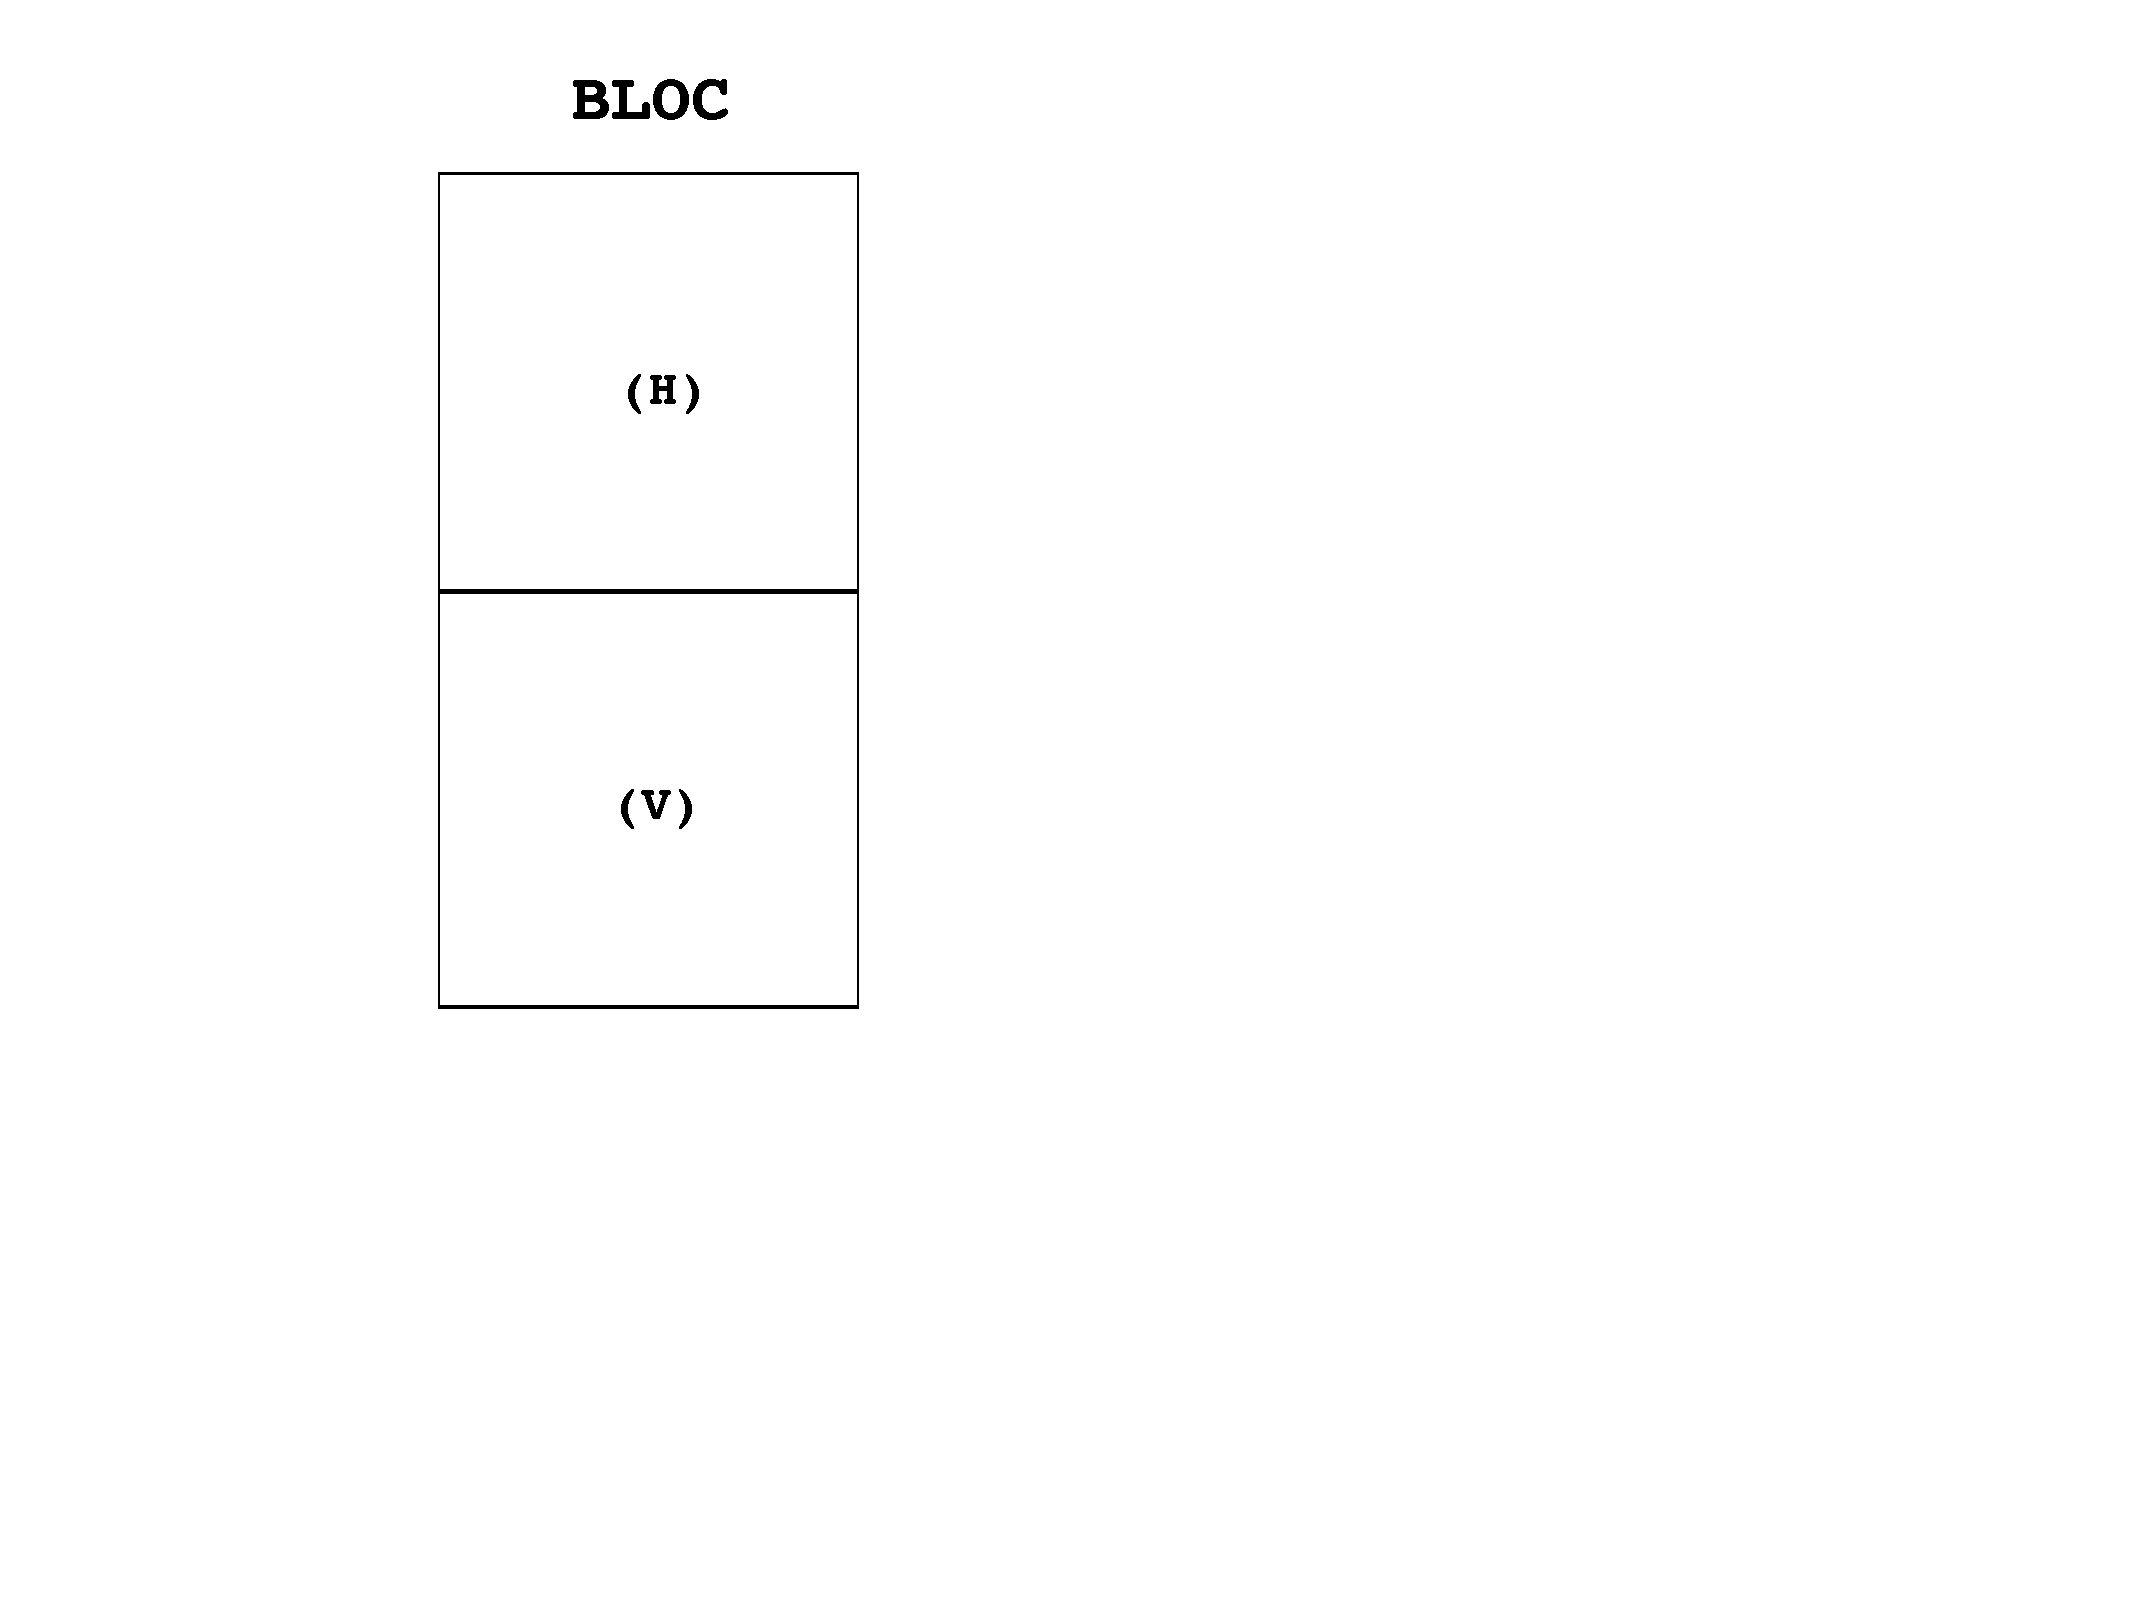
\includegraphics[height=1.8in]{BLOC.pdf}
	\end{subfigure}
	\caption*{Element-local system.}
\end{figure}
\end{minipage}

\vskip 5pt
\begin{minipage}[t]{0.60\textwidth}
Recall the statically condensed system\\[-5pt]
(cf.~Appendix~\ref{chap:dpg}): \vspace{-10pt}
\[
	\left[ \begin{array}{cc}
		\mr{B^* G^{-1} B} & \mr{B^* G^{-1} \hat B} \\
		\mr{\hat B^* G^{-1} B} & \mr{\hat B^* G^{-1} \hat B} \\
	\end{array} \right]
	\left[ \begin{array}{c}
		\mr{u_h} \\
		\mr{\hat u_h} 
	\end{array} \right]
	=
	\left[ \begin{array}{c}
		\mr{B^* G^{-1} l} \\
		\mr{\hat B^* G^{-1} l}
	\end{array} \right]
\]
\end{minipage}
\begin{minipage}[t]{0.39\textwidth}
Auxiliary local variables: \vspace{-10pt}
\begin{itemize}
	\itemsep -8pt
	\item \var{stiff\_HH} $\leftarrow \mr B$
	\item \var{stiff\_HV} $\leftarrow \mr{\hat B}$
	\item \var{bload\_H} $\leftarrow \mr l$
	\item \var{stiff\_ALL} $\leftarrow \left[ \mr{B \, | \, \hat B \, | \, l \, } \right]$
\end{itemize}
\end{minipage}

\vskip 5pt

In the \routine{elem} routine, these steps are implemented as follows:
\begin{enumerate}
	\item{ Preliminary set up:
\begin{lstlisting}[mathescape,caption=\file{POISSON/PRIMAL\_DPG/}\routine{elem}: preliminary set up]
!..allocate auxiliary matrices
   allocate(gramP(NrTest*(NrTest+1)/2))
   allocate(stiff_HH(NrTest,NrdofH))
   allocate(stiff_HV(NrTest,NrdofVi))
   allocate(bload_H(NrTest))

!..determine element type; number of vertices, edges, and faces
   etype = NODES(Mdle)%ntype
   nrv = nvert(etype); nre = nedge(etype); nrf = nface(etype)
   
!..determine order of approximation (element integrals)
   call find_order(Mdle, norder)
!..determine enriched order of approximation (hexa)
   nordP = NODES(Mdle)%order+NORD_ADD*111

!..determine edge and face orientations
   call find_orient(Mdle, norient_edge,norient_face)
!..determine nodes coordinates
   call nodcor(Mdle, xnod)
   
!  ....... element integrals
\end{lstlisting}
	}
	\item{ Element integration:
\begin{lstlisting}[mathescape,caption=\file{POISSON/PRIMAL\_DPG/}\routine{elem}: element integration]
!..use the enriched order to set the quadrature
   INTEGRATION = NORD_ADD ! $\Delta p \in \{1, 2, \ldots \}$
   call set_3D_int_DPG(etype,norder,norient_face, nrint,xiloc,waloc)

!..loop over integration points
   do l=1,nrint
!  ...coordinates and weight of this integration point
      xi(1:3) = xiloc(1:3,l); wa = waloc(l)

!  ...H1 shape functions (for geometry)
      call shape3DH(etype,xi,norder,norient_edge,norient_face, nrdofH,shapH,gradH)
!  ...discontinuous H1 shape functions
      call shape3HH(etype,xi,nordP, nrdof,shapHH,gradHH)

!  ...geometry map
      call geom3D(Mdle,xi,xnod,shapH,gradH,nrdofH, x,dxdxi,dxidx,rjac,iflag)
!  ...integration weight
      weight = rjac*wa
!  ...get the RHS
      call getf(Mdle,x, fval)

!  ...1st loop through enriched H1 test functions
      do k1=1,nrdofHH
!     ...Piola transformation
         v = shapHH(k1)
         dv(1:3) = gradHH(1,k1)*dxidx(1,1:3) + &
                    gradHH(2,k1)*dxidx(2,1:3) + &
                    gradHH(3,k1)*dxidx(3,1:3)
!
!     ...accumulate load: $(f,v)$
         bload_H(k1) = bload_H(k1) + fval*v*weight
!
!     ...loop through H1 trial functions
         do k2=1,nrdofH
!        ...Piola transformation
            dp(1:3) = gradH(1,k2)*dxidx(1,1:3) + &
                       gradH(2,k2)*dxidx(2,1:3) + &
                       gradH(3,k2)*dxidx(3,1:3)
!
!        ...accumulate stiffness: $(\nabla u, \nabla_h v)$
            stiff_HH(k1,k2) = stiff_HH(k1,k2) + weight*(dv(1)*dp(1)+dv(2)*dp(2)+dv(3)*dp(3))
         enddo

!     ...2nd loop through enriched H1 test functions for Gram matrix
         do k2=k1,nrdofHH
!        ...Piola transformation
            q = shapHH(k2)
            dq(1:3) = gradHH(1,k2)*dxidx(1,1:3) + & 
                       gradHH(2,k2)*dxidx(2,1:3) + &
                       gradHH(3,k2)*dxidx(3,1:3)

!        ...determine index in triangular packed format
            k = (k2-1)*k2/2+k1
!
!        ...accumulate Gram with test inner product: $(v,v)_\test := (v,v) + (\nabla_h v, \nabla_h v)$
            aux = q*v + (dq(1)*dv(1) + dq(2)*dv(2) + dq(3)*dv(3))
            gramP(k) = gramP(k) + aux*weight
         enddo; enddo; enddo
\end{lstlisting}
	}
	\item{ Boundary integration:
\begin{lstlisting}[mathescape,caption=\file{POISSON/PRIMAL\_DPG/}\routine{elem}: boundary integration.]
!..determine order of approximation (boundary integrals)
   norderi(1:nre+nrf) = norder(1:nre+nrf)
   norderi(nre+nrf+1) = 111

!..loop through element faces
   do ifc=1,nrf

!  ...sign factor to determine the outward normal unit vector
      nsign = nsign_param(etype,ifc)

!  ...face type ('tria','quad')
      ftype = face_type(etype,ifc)

!  ...face order of approximation
      call face_order(etype,ifc,norder, norderf)

!  ...set 2D quadrature
      INTEGRATION = NORD_ADD ! $\Delta p$
      call set_2D_int_DPG(ftype,norderf,norient_face(ifc), nrint,tloc,wtloc)

!  ...loop through integration points
      do l=1,nrint

!     ...face coordinates
         t(1:2) = tloc(1:2,l)
!     ...face parametrization
         call face_param(etype,ifc,t, xi,dxidt)

!     ...determine discontinuous H1 shape functions
         call shape3HH(etype,xi,nordP, nrdof,shapHH,gradHH)
!     ...determine element H(div) shape functions (for fluxes), interfaces only (no bubbles)
         call shape3DV(etype,xi,norderi,norient_face, nrdof,shapV,divV)

!     ...determine element H1 shape functions (for geometry)
         call shape3DH(etype,xi,norder,norient_edge,norient_face, nrdof,shapH,gradH)
!     ...geometry map
         call bgeom3D(Mdle,xi,xnod,shapH,gradH,nrdofH,dxidt,nsign, &
                        x,dxdxi,dxidx,rjac,dxdt,rn,bjac)
!     ...integration weight
         weight = bjac*wtloc(l)

!     ...loop through enriched H1 test functions
         do k1=1,nrdofHH
            v = shapHH(k1)

!        ...loop through H(div) trial functions
            do k2=1,nrdofVi
!           ...Piola transformation
               s(1:3) = (dxdxi(1:3,1)*shapV(1,k2) + &
                          dxdxi(1:3,2)*shapV(2,k2) + &
                          dxdxi(1:3,3)*shapV(3,k2)) / rjac
!           ...normal component
               sn = s(1)*rn(1)+s(2)*rn(2)+s(3)*rn(3)
!
!           ...accumulate stiffness: $-\lb \sigma \cdot n, v \rb_{\Gamma_h}$
               stiff_HV(k1,k2) = stiff_HV(k1,k2) - sn*v*weight

            enddo; enddo ! end loop through trial / test functions
   enddo; enddo; ! end loop through integration points / faces
\end{lstlisting}
	}
	\item{ Construction of DPG linear system:
\begin{lstlisting}[mathescape,caption=\file{POISSON/PRIMAL\_DPG/}\routine{elem}: constructing DPG linear system.]
!---------------------------------------------------------------------
!  Construction of statically condensed DPG linear system
!---------------------------------------------------------------------

!..create auxiliary matrix for dense linear algebra
   allocate(stiff_ALL(NrTest,NrTrial+1))

!..Total test/trial DOFs of the element
   i = NrTest ; j1 = NrdofH ; j2 = NrdofVi

!..Copy stiffness and load into one matrix: $\text{\var{stiff\_ALL}} \leftarrow [ \mr{B \, | \, \hat B \, | \, l \, } ]$
   stiff_ALL(1:i,1:j1)          = stiff_HH(1:i,1:j1)
   stiff_ALL(1:i,j1+1:j1+j2) = stiff_HV(1:i,1:j2)
   stiff_ALL(1:i,j1+j2+1)       = bload_H(1:i)

   deallocate(stiff_HH,stiff_HV)

!..A. Compute Cholesky factorization of Gram Matrix, $\mr{G=U^T U \, (=LL^T)}$
   call DPPTRF('U',NrTest,gramP,info)
!
!..B. Solve triangular system to obtain $\mr{\tilde B,\ \text{i.e.~solve } (L \tilde B=)\, U^T \tilde B = [B \, | \, l]}$
   call DTPTRS('U','T','N',NrTest,NrTrial+1,gramP,stiff_ALL,NrTest,info)

   allocate(raloc(NrTrial+1,NrTrial+1)); raloc = ZERO

!..C. Matrix multiply: $\mr{B^T G^{-1} B \, (=\tilde B^T \tilde B)}$
   call DSYRK('U','T',NrTrial+1,NrTest,ZONE,stiff_ALL,NrTest,ZERO,raloc,NrTrial+1)

!..D. Fill lower triangular part of Hermitian matrix $\mr{\tilde B^T \tilde B}$
   do i=1,NrTrial
      raloc(i+1:NrTrial+1,i) = raloc(i,i+1:NrTrial+1)
   enddo

!..raloc has now all blocks of the stiffness and load:
!  $r_{\text{aloc}} = \var{ALOC(1,1)} \quad \var{ALOC(1,2)} \quad \var{BLOC(1)}$
!         $\, \var{ALOC(2,1)} \quad \var{ALOC(2,2)} \quad \var{BLOC(2)}$
\end{lstlisting}
	}
\end{enumerate}




%%%%%%%%%%%%%%%%%%%%%%%%%%%%%%%

%
%!TEX root = ../../../hp3D_user_guide.tex
%

%--------------------------------------------------------------------

\section{Linear Elasticity Problems}
\label{sec:elasticity}

%\subsection{Galerkin implementation}
%\label{subsec:elasticity-galerkin}

Linear elasticity will be added in a future version of the user manual.

%The general structure of the \file{ELASTICITY} application directory is similar to the implementation of previously discussed applications. This section only focuses on the specific aspects of implementing particular formulations of linear elasticity. We encourage reading Section~\ref{sec:poisson} on Poisson problems for additional discussion of problem implementations, in general.


%%%%%%%%%%%%%%%%%%%%%%%%%%%%%%%

%
%!TEX root = ../../../hp3D_user_guide.tex
%

%--------------------------------------------------------------------

\section{Helmholtz Problems}
\label{sec:helmholtz}

%\subsection{Galerkin implementation}
%\label{subsec:helmholtz-galerkin}

Helmholtz (linear acoustics) will be added in a future version of the user manual.

%The general structure of the \file{HELMHOLTZ} application directory is similar to the implementation of previously discussed applications. This section only focuses on the specific aspects of implementing particular formulations of the Helmholtz problem. We encourage reading Section~\ref{sec:poisson} on Poisson problems for additional discussion of problem implementations, in general.



%%%%%%%%%%%%%%%%%%%%%%%%%%%%%%%

%
%!TEX root = ../../../hp3D_user_guide.tex
%

%--------------------------------------------------------------------

\section{Maxwell Problems}
\label{sec:maxwell}

For time-harmonic Maxwell problems, the solution is complex-valued; the \hp3D library must therefore be compiled with preprocessing flag \code{\var{COMPLEX}=1}.

The general structure of the \file{MAXWELL} application directory is similar to the implementation of previously discussed applications. This section only focuses on the specific aspects of implementing particular formulations of the Maxwell problem. We encourage reading Section~\ref{sec:poisson} on Poisson problems for additional discussion of problem implementations, in general.


\begin{itemize}
\item
{
Linear time-harmonic Maxwell equations:
\begin{alignat*}{3}
	\curl \bs E + i \omega \mu \bs H
	&= \bs 0 &\quad \text{in } \Omega \, , \\
	\curl \bs H - (i \omega \eps + \sigma) \bs E 
	&= \bs J^{\text{imp}} &\quad \text{in } \Omega \, , \\
	\bs n \times \bs E &= \bs n \times \bs E_0 &\quad \text{on } \Gamma \, .
\end{alignat*}
}
\item
{
Curl--curl formulation:
\begin{alignat*}{3}
	\curl (\mu^{-1} \curl \bs E) - (\omega^2 \eps - i \omega \sigma) \bs E
	&= -i \omega \bs J^{\text{imp}}  &\quad \text{in } \Omega \, , \\
	\bs n \times \bs E &= \bs n \times \bs E_0 &\quad \text{on } \Gamma \, .
\end{alignat*}
}
\item
{
Classical variational formulation:
\[
\left\{
\begin{array}{lll}
	\bs E \in \Hcurl : \bs n \times \bs E = \bs n \times \bs E_0 \text{ on } \Gamma \, , \\[5pt]
	(\mu^{-1} \curl \bs E,\curl \bs F) - ((\omega^2 \eps - i \omega \sigma) \bs E, \bs F)
	= -i \omega (\bs J^{\text{imp}}, \bs F) \, , \\[5pt]
	\hfill
	\quad \bs F \in \Hcurl \, : \, \bs n \times \bs F = \bs 0 \text{ on } \Gamma \, .
\end{array}
\right.
\]
The formulation involves just one unknown $\bs E \in \Hcurl$, defined on the whole domain.
}
\end{itemize}

\subsection{Galerkin implementation}
\label{subsec:maxwell-galerkin}

The Galerkin FE implementation of the classical (curl-curl) variational problem is located in the application directory \file{problems/MAXWELL/GALERKIN}. In the remainder of this section, file paths may be given as relative paths within the application directory.

The physics input file defines the vector-valued unknown: electric field $\bs E \in \Hcurl$.
\begin{lstlisting}[caption=\file{MAXWELL/GALERKIN/input/physics} input file.]
100000              MAXNODS, nodes anticipated
1                   NR_PHYSA, physics attributes
field  tangen  1    H(curl) variable
\end{lstlisting}

The curl-curl formulation above specifies a non-homogeneous Dirichlet boundary condition for the tangential component of the electric field. When setting a Dirichlet flag for an $H(\tcurl)$-variable in the \routine{set\_initial\_mesh} routine, the code automatically interprets the BC to be applied to the tangential component. As in previous examples, the values of the field and its derivative on the boundary must be supplied by the user in the \routine{dirichlet} routine.

The \routine{elem} routine for the Galerkin implementation of the Maxwell problem is given by the following code:

\begin{lstlisting}[mathescape,caption=\file{MAXWELL/GALERKIN/}\routine{elem} routine]
!..determine element type
   etype = NODES(Mdle)%ntype
   
!..determine order of approximation
   call find_order(Mdle, norder)
   
!..determine edge and face orientations
   call find_orient(Mdle, norient_edge,norient_face)
   
!..determine nodes coordinates
   call nodcor(Mdle, xnod)
   
!..set quadrature points and weights
   call set_3D_int(etype,norder,norient_face, nrint,xiloc,waloc)

!  ....... element integrals:

!..loop over integration points
   do l=1,nrint

!  ...coordinates and weight of this integration point
      xi(1:3) = xiloc(1:3,l); wa = waloc(l)

!  ...H1 shape functions (for geometry)
      call shape3DH(etype,xi,norder,norient_edge,norient_face, nrdofH,shapH,gradH)

!  ...H(curl) shape functions
      call shape3DE(etype,xi,norder,norient_edge,norient_face, nrdofE,shapE,curlE)

!  ...geometry map
      call geom3D(Mdle,xi,xnod,shapH,gradH,nrdofH, x,dxdxi,dxidx,rjac,iflag)

!  ...integration weight
      weight = rjac*wa

!  ...get the RHS (complex, vector-valued)
      call getf(Mdle,x, zJ)

!  ...loop through H(curl) test functions
      do k1=1,nrdofE

!     ...Piola transformation: $F \rightarrow J^{-T} \hat F$ and $\curl F \rightarrow (\det J)^{-1} J \, \hat \nabla \times \hat F$
         F(1:3) = shapE(1,k1)*dxidx(1,1:3) &
                 + shapE(2,k1)*dxidx(2,1:3) &
                 + shapE(3,k1)*dxidx(3,1:3)
         CF(1:3) = ( dxdxi(1:3,1)*curlE(1,k1) &
                    + dxdxi(1:3,2)*curlE(2,k1) &
                    + dxdxi(1:3,3)*curlE(3,k1) ) / rjac

!     ...accumulate for the load vector: $(-i \omega J,F)$
         za = F(1)*zJ(1) + F(2)*zJ(2) + F(3)*zJ(3)
         Zbloc(k1) = Zbloc(k1) - ZI*OMEGA*za*weight

!     ...loop through H(curl) trial functions
         do k2=1,nrdofE

!        ...Piola transformation: $E \rightarrow J^{-T} \hat E$ and $\curl E \rightarrow (\det J)^{-1} J \, \hat \nabla \times \hat E$
            E(1:3) = shapE(1,k2)*dxidx(1,1:3) &
                    + shapE(2,k2)*dxidx(2,1:3) &
                    + shapE(3,k2)*dxidx(3,1:3)
            CE(1:3) = ( dxdxi(1:3,1)*curlE(1,k2) &
                       + dxdxi(1:3,2)*curlE(2,k2) &
                       + dxdxi(1:3,3)*curlE(3,k2) ) / rjac

!        ...accumulate for the stiffness matrix: $((1/\mu) \tcurl E, \tcurl F)-((\omega^2 \eps - i \omega \sigma) E, F)$
            za = (CE(1)*CF(1) + CE(2)*CF(2) + CE(3)*CF(3)) / MU
            zb = (OMEGA*OMEGA*EPS - ZI*OMEGA*SIGMA) * (E(1)*F(1) + E(2)*F(2) + E(3)*F(3))
            Zaloc(k1,k2) = Zaloc(k1,k2) + (za-zb)*weight

   enddo; enddo; enddo
\end{lstlisting}

%--------------------------------------------------------------------
\subsection{DPG ultraweak implementation}
\label{sec:maxwell-ultraweak}

The broken ultraweak Maxwell formulation is given by:
\[
\left\{
\begin{split}
	\bs E, \bs H \in \bs{L^2}(\Omega), \hat{\bs E}, \hat{\bs H} \in H^{-1/2}(\tcurl, \Gammah): \bs n \times \bs E &= \bs n \times \bs E_0 \text{ on } \Gamma \, , \\
	(\bs H, \hcurl \bs F) - ((i \omega \eps + \sigma) \bs E , \bs F)
	&= (\bs J^{\text{imp}}, \bs F) &\quad \bs F \in \hHcurl \, , \\
	(\bs E, \hcurl \bs G) + \lb \bs n \times \hat{\bs E}, \bs G \rb_{\Gammah} + (i \omega \mu \bs H, \bs G)
	&= \bs 0 &\quad \bs G \in \hHcurl \, .
\end{split}
\right .
\]

Before looking at this section, the reader is encouraged to review the simpler DPG implementations of the Poisson problem, given in Sections~\ref{sec:poisson-primal} (primal) and \ref{sec:poisson-ultraweak} (ultraweak), which are discussed in greater detail. As in the Poisson DPG implementation, the static condensation of the Riesz representation of the residual is done at the element level (cf.~Section~\ref{sec:poisson-primal}). This model problem implementation uses a scaled adjoint graph norm for the ultraweak Maxwell formulation:
\[
	\| ( \bs F, \bs G ) \|^2_\test :=
	\| \hcurl \bs F - i \omega \bar{\mu} \bs G \|^2 +
	\| \hcurl \bs G + (i \omega \bar{\eps} - \sigma) \bs F \|^2 +
	\alpha ( \| \bs F \|^2 + \| \bs G \|^2) \, ,
\]
where $\bar{\cdot}$ indicates complex-conjugate, and $\alpha > 0$ is a scaling constant. See, e.g., \cite{melenk2023waveguide1, demkowicz2023waveguide2}, for both theoretical considerations and practical implications in terms of stability of choosing a proper value for $\alpha$.

The implementation is provided in \file{problems/MAXWELL/ULTRAWEAK\_DPG}.

\begin{lstlisting}[caption=\file{MAXWELL/ULTRAWEAK\_DPG/input/physics} input file.]
100000              MAXNODS, nodes anticipated
2                   NR_PHYSA, physics attributes
EHtrc   tangen 2    traces of electric/magnetic fields, H(curl), 2 components
EHfld   discon 6    electric/magnetic fields, L2, 3+3 components
\end{lstlisting}

In the ultraweak formulation, there are four physics unknowns: $\hat{\bs E}$, $\hat{\bs H}$, $\bs E$, $\bs H$; however, since all physics variables are solved in the same formulation and the electric and magnetic fields (and their traces) each use the same respective energy spaces (namely $\bs{L^2}$ and $H^{-1/2}(\tcurl)$), one can alternatively group these variables by specifying only two physics variables with double the number of components each: $(\hat{\bs E},\hat {\bs H}) \in (H^{-1/2}(\tcurl, \Gammah))^2$ and $(\bs E, \bs H) \in (\bs{L^2}(\Omega))^2$---recall that $\bs{L^2}(\Omega) = (L^2(\Omega))^3$. The variables are defined in the \file{physics} file and the tangential traces $(\hat{\bs E},\hat {\bs H})$ are specified as such by setting \code{\var{PHYSAi(1)}=.true.}. Choosing to specify grouped physics variables in such a way has certain implications for the ordering of degrees of freedom and the allocation of element-local matrices \var{ALOC} and \var{BLOC} (see Section~\ref{sec:coupled-variables}).

The element integration routine for the ultraweak DPG formulation is given by the following code:
\begin{lstlisting}[mathescape,caption=\file{MAXWELL/ULTRAWEAK\_DPG/}\routine{elem\_maxwell}: element integration]
!  ...use the enriched order to set the quadrature
      INTEGRATION = NORD_ADD
      call set_3D_int_DPG(ntype,norder,norient_face, nrint,xiloc,waloc)

!  ...loop over integration points
      do l=1,nrint

!     ...coordinates and weight of this integration point
         xi(1:3)=xiloc(1:3,l); wa=waloc(l)

!     ...H1 shape functions (for geometry)
         call shape3DH(ntype,xi,norder,norient_edge,norient_face, nrdofH,shapH,gradH)

!     ...L2 shape functions for the trial space
         call shape3DQ(ntype,xi,norder, nrdofQ,shapQ)

!     ...broken H(curl) shape functions for the enriched test space
         call shape3EE(ntype,xi,nordP, nrdofEE,shapEE,curlEE)

!     ...geometry map
         call geom3D(Mdle,xi,xnod,shapH,gradH,nrdofH, x,dxdxi,dxidx,rjac,iflag)

!     ...get permittivity at x
         call get_permittivity(mdle,x, eps)

!     ...integration weight
         weight = rjac*wa

!     ...get the RHS
         call getf(Mdle,x, zJ)

!     ...permittivity
         za = (ZI*OMEGA*EPS) * eps(:,:)

!     ...scalar permeability
         zc1 = ZI*OMEGA*MU

!     ...apply pullbacks
         call DGEMM('T','N',3,nrdofEE,3,1.d0     ,dxidx,3,shapEE,3,0.d0,shapF,3)
         call DGEMM('N','N',3,nrdofEE,3,1.d0/rjac,dxdxi,3,curlEE,3,0.d0,curlF,3)

!     ...apply permittivity
         zshapF = cmplx(shapF,0.d0,8)
         zcurlF = cmplx(curlF,0.d0,8)
         call ZGEMM('C','N',3,nrdofEE,3,ZONE,za,3,zshapF,3,ZERO,epsTshapF,3)
         call ZGEMM('N','N',3,nrdofEE,3,ZONE,za,3,zcurlF,3,ZERO,epscurlF ,3)

!     ...loop through enriched H(curl) test functions
         do k1=1,nrdofEE

!        ...pickup pulled-back test functions
            fldF(:) = shapF(:,k1);  crlF(:) = curlF(:,k1)
            fldG(:) = fldF(:);      crlG(:) = crlF(:)
            epsTfldF(:) = epsTshapF(:,k1)

!  --- load ---
!           $(J^{\text{imp}}, F)$ first equation RHS (with first H(curl) test function F)
!           $(0, G)$ second equation RHS is zero
            n = 2*k1-1
            bload_E(n) = bload_E(n) + (fldF(1)*zJ(1)+fldF(2)*zJ(2)+fldF(3)*zJ(3)) * weight

!  --- stiffness matrix ---
!        ...loop through L2 trial shape functions
            do k2=1,nrdofQ
!           ...first L2 variable
               m = (k2-1)*6
!           ...Piola transformation
               fldE(1:3) = shapQ(k2)/rjac; fldH = fldE

!           ...$-i \omega \eps (E,F)$
!           ...$(H,\curl F)$
               n = 2*k1-1
               stiff_EQ_T(m+1:m+3,n) = stiff_EQ_T(m+1:m+3,n) - fldE(:)*conjg(epsTfldF(:))*weight
               stiff_EQ_T(m+4:m+6,n) = stiff_EQ_T(m+4:m+6,n) + fldH(:)*crlF(:)*weight

!           ...$(E, \curl G)$
!           ...$i \omega \mu (H,G)$
               n = 2*k1
               stiff_EQ_T(m+1:m+3,n) = stiff_EQ_T(m+1:m+3,n) + fldE(:)*crlG(:)*weight
               stiff_EQ_T(m+4:m+6,n) = stiff_EQ_T(m+4:m+6,n) + zc1*fldH(:)*fldG(:)*weight
            enddo !..end of loop through L2 trial functions

!  --- Gram matrix ---
!        ...loop through enriched H(curl) test functions
            do k2=k1,nrdofEE
               fldE(:) = shapF(:,k2); epsTfldE(:) = epsTshapF(:,k2)
               crlE(:) = curlF(:,k2); epscrlE(:) = epscurlF(:,k2)

               call dot_product(fldF,fldE, FF)
               call dot_product(crlF,crlE, CC)

!          ...accumulate for the Hermitian Gram matrix (compute upper triangular only)
!             ------------------------
!             | (F_i,F_j)   (F_i,G_j) |    F_i/G_i are outer loop shape functions (fldF)
!             | (G_i,F_j)   (G_i,G_j) |    F_j/G_j are inner loop shape functions (fldE)
!             ------------------------

!             (F_j,F_i) terms = Int[F_^*i F_j] terms (G_11)
               n = 2*k1-1; m = 2*k2-1; k = nk(n,m)
               zaux = conjg(epsTfldF(1))*epsTfldE(1) + &
                       conjg(epsTfldF(2))*epsTfldE(2) + &
                       conjg(epsTfldF(3))*epsTfldE(3)
               gramP(k) = gramP(k) + (zaux + ALPHA_NORM*FF + CC)*weight

!              (G_j,F_i) terms = Int[F_^*i G_j] terms (G_12)
               n = 2*k1-1; m = 2*k2; k = nk(n,m)
               zaux = -(fldF(1)*epscrlE(1) + fldF(2)*epscrlE(2) + fldF(3)*epscrlE(3))
               zcux = conjg(zc1)*(crlF(1)*fldE(1) + crlF(2)*fldE(2) + crlF(3)*fldE(3))
               gramP(k) = gramP(k) + (zaux+zcux)*weight

!           ...compute lower triangular part of 2x2 G_ij matrix
!              only if it is not a diagonal element, G_ii
               if (k1 .ne. k2) then
!                 (F_j,G_i) terms = Int[G_^*i F_j] terms (G_21)
                  n = 2*k1; m = 2*k2-1; k = nk(n,m)
                  zaux = -(crlF(1)*epsTfldE(1) + crlF(2)*epsTfldE(2) + crlF(3)*epsTfldE(3))
                  zcux = zc1*(fldF(1)*crlE(1) + fldF(2)*crlE(2) + fldF(3)*crlE(3) )
                  gramP(k) = gramP(k) + (zaux+zcux)*weight
               endif

!              (G_j,G_i) terms = Int[G_^*i G_j] terms (G_22)
               n = 2*k1; m = 2*k2; k = nk(n,m)
               zcux = abs(zc1)**2*(fldF(1)*fldE(1) + fldF(2)*fldE(2) + fldF(3)*fldE(3))
               gramP(k) = gramP(k) + (zcux + ALPHA_NORM*FF + CC)*weight
         enddo; enddo !..end of loop through enriched H(curl) test functions
      enddo !..end of loop through integration points
\end{lstlisting}

Next, we provide the code performing the boundary integration:
\begin{lstlisting}[mathescape,caption=\file{MAXWELL/ULTRAWEAK\_DPG/}\routine{elem\_maxwell}: boundary integration]
!  ...loop through element faces
      do ifc=1,nrf

!     ...sign factor to determine the outward normal unit vector
         nsign = nsign_param(ntype,ifc)

!     ...face type
         ftype = face_type(ntype,ifc)

!     ...face order of approximation
         call face_order(ntype,ifc,norder, norderf)

!     ...set 2D quadrature
         INTEGRATION = NORD_ADD
         call set_2D_int_DPG(ftype,norderf,norient_face(ifc), nrint,tloc,wtloc)

!     ...loop through integration points
         do l=1,nrint

!        ...face coordinates
            t(1:2) = tloc(1:2,l)

!        ...face parametrization
            call face_param(ntype,ifc,t, xi,dxidt)

!        ...determine discontinuous H(curl) shape functions
            call shape3EE(ntype,xi,nordP, nrdof,shapEE,curlEE)

!        ...determine element H1 shape functions (for geometry)
            call shape3DH(ntype,xi,norder,norient_edge,norient_face, nrdof,shapH,gradH)

!        ...determine element H(curl) shape functions (for fluxes) on face
            call shape3DE(ntype,xi,norderi,norient_edge,norient_face, nrdof,shapE,curlE)

!        ...geometry map
            call bgeom3D(Mdle,xi,xnod,shapH,gradH,NrdofH,dxidt,nsign, &
                          x,dxdxi,dxidx,rjac,dxdt,rn,bjac)
            weight = bjac*wtloc(l)

!        ...pullback trial and test functions
            call DGEMM('T','N',3,nrdofEE,3,1.d0,dxidx,3,shapEE,3,0.d0,shapF ,3)
            call DGEMM('T','N',3,nrdofEi,3,1.d0,dxidx,3,shapE ,3,0.d0,shapFi,3)

!        ...loop through enriched H(curl) test functions
            do k1=1,nrdofEE
               E1(1:3) = shapF(:,k1)

!           ...loop through H(curl) trial functions
               do k2=1,NrdofEi
                  E2(1:3) = shapFi(:,k2)
                  call cross_product(rn,E2, rntimesE)

                  stiff_EE_T(2*k2-1,2*k1) = stiff_EE_T(2*k2-1,2*k1) + &
                              weight*( E1(1)*rntimesE(1) + E1(2)*rntimesE(2) + E1(3)*rntimesE(3) )
               enddo !..end loop through H(curl) trial functions
            enddo !..end loop through the enriched H(curl) test functions
         enddo !..end loop through integration points
      enddo !..end loop through element faces
\end{lstlisting}

Finally, the code performing the construction of the DPG linear system:
\begin{lstlisting}[mathescape,caption=\file{MAXWELL/ULTRAWEAK\_DPG/}\routine{elem\_maxwell}: constructing DPG linear system.]
      allocate(stiff_ALL(NrTest,NrTrial+1))

!  ...Total test/trial DOFs of the element
      i1 = NrTest ; j1 = 2*NrdofEi ; j2 = 6*NrdofQ

! ...Copy stiffness and load into one matrix
      stiff_ALL(1:i1,1:j1) = transpose(stiff_EE_T(1:j1,1:i1))
      stiff_ALL(1:i1,j1+1:j1+j2) = transpose(stiff_EQ_T(1:j2,1:i1))
      stiff_ALL(1:i1,j1+j2+1) = bload_E(1:i1)

!  ...A. Compute Cholesky factorization of Gram Matrix, $\mr{G=U^* U (=LL^*)}$
      call ZPPTRF('U',NrTest,gramP,info)

!  ...B. Solve triangular system to obtain $\mr{\tilde{B}}$, $\mr{(LX=) U^* X = [B|l]}$
      call ZTPTRS('U','C','N',NrTest,NrTrial+1,gramP,stiff_ALL,NrTest,info)

      allocate(zaloc(NrTrial+1,NrTrial+1)); zaloc = ZERO

!  ...C. Matrix multiply: $\mr{B^* G^{-1} B (=\tilde{B}^* \tilde{B})}$
      call ZHERK('U','C',NrTrial+1,NrTest,ZONE,stiff_ALL,NrTest,ZERO,zaloc,NrTrial+1)

!  ...D. Fill lower triangular part of Hermitian matrix $\mr{\tilde B^* \tilde B}$
      do i=1,NrTrial
         zaloc(i+1:NrTrial+1,i) = conjg(zaloc(i,i+1:NrTrial+1))
      enddo

!..zaloc has now all blocks of the stiffness and load:
!  $z_{\text{aloc}} =  \var{ALOC(1,1)} \quad \var{ALOC(1,2)} \quad \var{BLOC(1)}$
!         $\, \var{ALOC(2,1)} \quad \var{ALOC(2,2)} \quad \var{BLOC(2)}$
\end{lstlisting}






%%%%%%%%%%%%%%%%%%%%%%%%%%%%%%%

%\section*{Historical Comments}



